\section{Численные методы решения}
\label{sec:algrhtms}

Далее мы опишем алгоритмы использующиеся для решений уравнений
эйконала. Это два разных метода, базирующиеся на разных и идеях и,
следовательно, пригодные для разных целей. Один заточен для
максимального ускорения работы и, как это часто бывает с такими
алгоритмами практически неспособен к параллелизации, другой же --
наоборот работает несколько медленнее, но гораздо проще поддается
распараллеливанию.

\subsection{Общая идея методов}
\label{sec:general-idea}

Для всех методов нам необходимо научится решать задачу в локальном
случае. Разберем для начала одномерный случай. Пусть нам дано
следующее уравнение эйконала:

\begin{equation}
  \label{eq:eik_smp}
  \sqrt{(\frac{dT}{dx})^2}=F(x), T(-1) = T(1) = 0.
\end{equation}


% Вставить куда-нибудь ссылку
Для упрощения обозначений мы запишем производную $T$ по $x$ в виде
$T_x$. Также в будущем мы будем поступать и для частных
производных. После преобразования уравнение~\eqref{eq:eik_smp} примет вид:

\begin{equation*}
  \sqrt{T_x^2}=F(x), T(-1) = T(1) = 0.
\end{equation*}


Имеется функция скорости $F(x) > 0$, требуется построить
решение $T(x)$. Мы видим, что решение не уникально (если t(x) решает
задачу, то тогда и $-t(x)$ также ее решает). Будем работать только с
положительными решениями.

Рассмотрим обыкновенное дифференциальное уравнение и разобьем решение
на подзадачи:

\begin{equation*}
  \begin{cases}
      \begin{array}{ll}
        T_x = ~F(x), \quad x \ge 0,\\
        T_x = -F(x), \quad x \le 0,\\[0.3cm]
        T(-1)= T(1) = 0.
      \end{array}
    \end{cases}
\end{equation*}

Для численной аппроксимации разобьем ось $x$ на набор точек сетки
$x_i=i\Delta x$. Положим $T_i = T(i \Delta x)$ и $F_i = F(i \Delta
x)$, где $\Delta x$ - это шаг дискретизации, $i = -n, \cdots,
n$. 

введем также обозначение для разностных производных первого порядка 1-го порядка:

\begin{eqnarray*}
    D^{+x}_iT(x_i) &=& \frac{T_{i+1} - T_{i}}{\Delta x} \\
    D^{-x}_iT(x_i) &=& \frac{T_{i} - T_{i-1}}{\Delta x}
\end{eqnarray*}

Далее используем разложение Тейлора и отбросим остаток. Получим
следующую дискретную систему:


\begin{equation}
  \label{eq:discretise}
  \begin{cases}
      T_n = 0,\\
      D^{+x}_iT(x_i) = F_i, \quad i>0 \\
      D^{-x}_iT(x_i)  = F_i, \quad i>0\\
      T(-n) = 0\\
    \end{cases}
\end{equation}

Отметим, что
\begin{itemize}
\item[ ] $T_{n-1}$ может быть получено из $T_n$
\item[ ] $T_{n-2}$ может быть получено из $T_{n-1}$
\item[ ]  $\cdots$
\item[ ] $T_{1}$ может быть получено из $T_2$
\item[ ] $T_{0}$ может быть получено из $T_{1}$
\item[ ]  $\cdots$
\item[ ] $T_{-n+1}$ может быть получено из $T_{-n}$
\item[ ] $T_{-n+2}$ может быть получено из $T_{-n+1}$
\item[ ]  $\cdots$
\item[ ] $T_{-1}$ может быть получено из $T_{-2}$
\item[ ] $T_{0}$ может быть получено из $T_{-1}$

\end{itemize}

Выше мы построили разностную схему, где вычисляем производные двигаясь
по направлению распространения границы: каждое следующее уравнения вне
текущей границы получено на основании уже имеющихся решений внутри
нее.

Вычисляя уравнение эйконала мы видим, что информация распространяется
как волны с определенной скоростью вдоль направления градиента. Наш
метод дискретизации вычисляет значения переменных используя
направления того откуда информация о решениях приходит. Если говорить
точнее, то дискретизация уравнений в частных производных использует
конечно-разностную трассировку смещающуюся в направлении знака
градиента.

Для одномерного случая у нас есть только два направления для каждой
точки $i$: правое $(i+1)$ и левое $(i - 1)$. Предположим, что у нас
есть решение в точке $i$, на итерации с номером $n$. Тогда мы имеем
два случая:
\begin{itemize}
\item Правое направление: $T_i^{n+1} = T_i^n - \Delta x D^{+x}_iT(x_i)$
\item Левое направление: $T_i^{n+1} = T_i^n - \Delta x D^{-x}_iT(x_i)$
\end{itemize}


Подобным образом используя разложение Тейлора в $x$ и $y$ для
величины $T$ мы можем определить эти обозначения для двумерного
случая, задав тем самым регулярную двумерную сетку дискретизации,
тогда для точек $(x,y)$, с разбиением
$(x_i,y_i) = (i\Delta_x,j \Delta_y)$ и $T_{ij} = T(x_i,y_i)$ мы
получим:

\begin{equation}
  \begin{aligned}
  \label{eq:discrete-defines}
    D^{-x}_{i,j}T(x,y)& =& \frac{T_{i,j} - T_{i-1,j}}{\Delta_x}  \\
    D^{+x}_{i,j}T(x,y)& =& \frac{T_{i+1,j} - T_{i,j}}{\Delta_x}  \\
    D^{-y}_{i,j}T(x,y) &=& \frac{T_{i,j} - T_{i,j-1}}{\Delta_y}  \\
    D^{+y}_{i,j}T(x,y) &=& \frac{T_{i,j} - T_{i,j+1}}{\Delta_y}
    \end{aligned}
\end{equation}

\begin{itemize}
\item $D^{+x}$ вычисляет новое значение в узле сетки $(i,j)$ используя
  информацию из $i$ и $i+1$, таким образом информация для решения
  распространяется справа налево.

\item $D^{-x}$ вычисляет новое значение в узле сетки $(i,j)$ используя
  информацию из $i$ и $i-1$, таким образом информация для решения
  распространяется слева направо.
\item $D^{+y}$ вычисляет новое значение в узле сетки $(i,j)$ используя
  информацию из $j$ и $j+1$, таким образом информация для решения
  распространяется сверху вниз.

\item $D^{-y}$ вычисляет новое значение в узле сетки $(i,j)$ используя
  информацию из $j$ и $j-1$, таким образом информация для решения
  распространяется снизу вверх.

\end{itemize}

Для двумерного случая разностные схемы действуют вдоль направления
градиента. На рисунке~\ref{fig:upwind-schema} иллюстрируются две
возможных ситуации. В первом случае распространение информации идет из
третьего квадранта, В другом случае -- из второго
\begin{figure}[H]
  \centering
  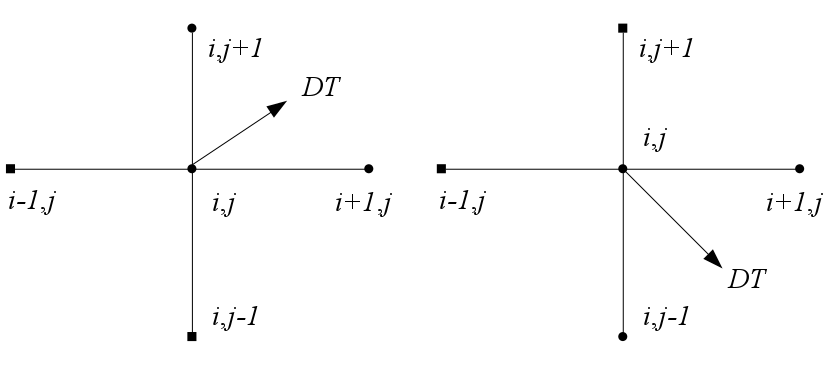
\includegraphics[width=\linewidth]{img/upwind-schema.png}
  \hfil \caption{Пример разных направлений распространения}
  \label{fig:upwind-schema}

\end{figure}

Крэндалл и Лайонс в \cite{V1983} доказали, что последовательные
монотонные схемы сходятся к корректному вязкостному решению. Поэтому
мы можем развивать идеи дальше и применить сказанное выше к уравнениям
эйконала. Существует несколько различных схем приближения, мы
воспользуемся схемой Годунова \cite{F2002}:

\begin{equation}
  \label{eq:godunov-schema}
  \begin{cases}
    \begin{matrix}
       &\max (D^{-x}_{ij}T, -D^{x}_{ij},0)^2 &+\\
     + &\max (D^{-y}_{ij}T, -D^{y}_{ij},0)^2&
    \end{matrix}
    \end{cases}= \frac{1}{F_{ij}^2}
\end{equation}

% Рассмотрим, как будет работать схема Годунова на простом примере:
% $\Delta x = 1$ и $F(x) = 1, 1 < i < n$ и покажем, что она выделяет
% только вогнутые решения:


% Как мы можем решить уравнение \eqref{eq:godunov-schema}? Предположим,
% что у нас есть сетка. Рассмотрим один ее узел и 4 ближайших ее соседа
% см. рисунок~\ref{fig:rec-grid-node}

% \begin{figure}[ht]
%   \centering
%   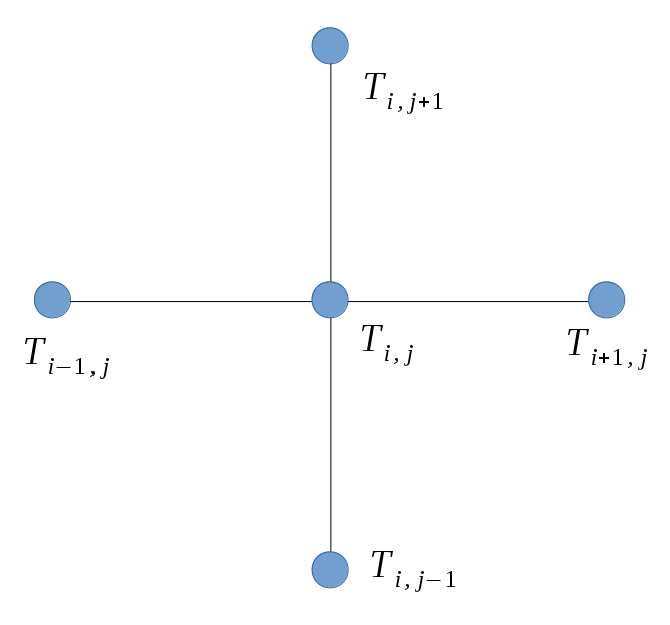
\includegraphics[width=0.5\linewidth]{img/rec-grid-node.png}
%   \hfil \caption{Узлы сетки}
%   \label{fig:rec-grid-node}

% \end{figure}

% Нам нужно выяснить значение $T_{i,j}$. Если исходить из оговоренных в
% постановке задачи условий, хотя бы одна из соседних точек имеет
% числовое значение,

Далее мы подставляем наши разностные производные
\eqref{eq:discrete-defines} в схему Годунова \eqref{eq:godunov-schema}
и получим

\begin{equation}
  \begin{aligned}
  \label{eq:replaced}
    T &= T_{i,j}\\
    T_{x}&= \min(T_{i-1,j},T_{i+1,j})\\
    T_{y}&= \min(T_{i,j-1},T_{i,j-1})
      \end{aligned}
\end{equation}

Уравнение эйконала может быть переписано для дискретного двумерного
случая на прямоугольной сетке как
\begin{equation*}
  \sqrt{\max \left( \frac {T-T_{x}}{\Delta_x},0 \right)^2+  \max \left( \frac
  {T-T_{y}}{\Delta_y},0\right)^2} = \frac{1}{F_{i,j}}
\end{equation*}
Или эквивалентно, можем записать:
\begin{equation}
  \label{eq:discrete-eikonal}
  \max \left( \frac {T-T_{x}}{\Delta_x},0 \right)^2+  \max \left( \frac
      {T-T_{y}}{\Delta_y},0\right)^2 = \frac{1}{F_{i,j}^2}
\end{equation}

Поскольку предполагается, что скорость распространения фронта
положительная $(F>0)$, $T$ будет больше чем $T_x$ и $T_y$ когда фронт
еще не посещал точку $(i,j)$. Следовательно уравнение
\eqref{eq:discrete-eikonal} можно безболезненно переписать еще раз:

\begin{equation}
  \label{eq:discrete-eikonal-2}
  \left( \frac {T-T_{x}}{\Delta_x} \right)^2+
  \left( \frac {T-T_{y}}{\Delta_y} \right)^2 = \frac{1}{F_{i,j}^2}
\end{equation}

Уравнение \eqref{eq:discrete-eikonal-2} обычное квадратное уравнение
вида $aT^2+bT+c=0$ где:

\begin{equation}
  \begin{aligned}
  \label{eq:replaced}
    a &= \Delta_2 x + \Delta^2 y\\[0.4cm]
    b &= -2(\Delta^2y T_{x}+\Delta^2x T_{y})\\
    c &= \Delta^2 y T_{y}^2 + \Delta^2 x T_{x}^2 - \frac{\Delta^2 x
      \Delta^2 y}{F_{ij}^2}
    \end{aligned}
\end{equation}


\subsection{Fast marching method на прямоугольной сетке}
\label{sec:fast-marching-method}

Fast marching method (FMM) \cite{S1999} является наиболее
распространенным способом решать уравнения эйконала. По своей
структуре он сильно похож на алгоритм Дейкстры. Главное отличие от
этого алгоритма в том алгоритм Дейкстры работает на
графе. Следовательно значение каждого узла $x_i$ зависит только от
родительского узла ${x_j}$, следуя принципу оптимальности Белмана.
\begin{equation*}
  T_i = \min_{x_i\in \mathcal{N}} (c_{ij} + T_j)
\end{equation*}

Другими словами узел $x_i$ присоединенный к $x_j$ в его
окрестности $\mathcal{N}(x_i)$ минимизирует (или
максимизирует) значение функции (в этом случае $T_i$)состоящей в
значении функции $T_j$ плюс добавленная стоимость движения из $x_j$ в
$x_i$, представленной как $c_{ij}$.
FMM также следует принципу оптимальности Белмана, но значения для
каждого узла получается из дискретизации уравнения Эйконала,
описанного выше. Эта дискретизация учитывает при подсчитывании
значения всех соседей, поэтому в непрерывном случае FMM вычисляет
время прибытия более аккуратно.

Алгоритм помечает ячейки тремя различными метками:
\begin{list}{}{}
\item \textbf{Изведанная} : значение в этой ячейке не подлежит более
  пересмотру,
\item \textbf{Неизведанная} : ячейка, значение в которой еще не
  получено,
\item \textbf{Пробная}: лежит на границе между \textbf{Изведанными}
  и \textbf{Неизведанными} ячейками, значения функции в этих ячейках
  уже известны, но не определены.
\end{list}

Процедура описанная ниже инициализирует все точки в сетке в состояние
\textbf{Неизведанное} c бесконечным временем достижения. Стартовые
точки устанавливаются в $0$ и считаются \textbf{Изведанными}. Далее основной
цикл FMM начинает выбирать узлы с наименьшим временем прибытия из
\textbf{Пробных} узлов. Для всех соседей этого узла, не являющихся
\textbf{Изведанными} решается уравнение эйконала и получается новое
значение времени прибытия. Если оно оказалось меньше чем текущее
значение, то оно заменяет старое. Если соседняя точка была
\textbf{Неизведанной}, то она становится пробной. Наконец, выбранная
точка становится \textbf{Изведанной} и начинается новая итерация
алгоритма, пока у нас существуют \textbf{Пробные} точки. Полученная
сетка, где в каждой точке наименьшее возможное время прибытия в нее
является результатом работы алгоритма


\subsection{Fast sweeping method на прямоугольной сетке}
\label{sec:fast-sweeping-method}

Fast sweeping method (метод быстрых выметаний. обычно даже в
русских публикациях не переводится) далее FSM -- итеративный метод, который
использует разностную схему для дискретизации уравнения эйконала
\cite{F2005}. Идея, скрывающаяся за FSM это ``замести'' сетку в
определенных направлениях. Порядок выметания определяется
характеристиками соответствующего уравнения эйконала

\subsection{Fast sweeping method на нерегулярной сетке}
\label{sec:unstructured-mesh}

\subsubsection{Триангуляция}
\label{sec:triangulate}

\subsection{Вопросы реализации}
\label{sec:programming}



%%% Local Variables:
%%% mode: latex
%%% TeX-master: "eikonal_solver"
%%% End:
